
\documentclass[12pt,a4paper]{extarticle}
\usepackage{unicode-math}
\usepackage{luatextra}
\defaultfontfeatures{Renderer=Basic, Ligatures=TeX}
\usepackage{ifxetex}
\usepackage{ifluatex}
\usepackage{graphicx}
%\usepackage[english,russian]{babel}
\usepackage{polyglossia}
\usepackage{hyperref}
\usepackage{tikz}
\usepackage{microtype}
\tikzset{node distance=4em, auto}

\ifluatex
  \usepackage{pdftexcmds}
  \makeatletter
  \let\pdfstrcmp\pdf@strcmp
  \let\pdffilemoddate\pdf@filemoddate
  \makeatother
\fi
\usepackage{svg}
% \setsvg{inkscape={"/usr/bin/inkscape"= -z -C}}
\setsvg{inkscape = inkscape -z -D}

% \fontspec{Free Serif}  % Good Times-like
% \setmainfont{CharisSIL} % Russian italik weird.
% \setmainfont{Fira Sans}
% \setmainfont{Free Serif}
\setmainfont{Libertinus Serif}
%\setmainfont{Pomorsky}
\setmonofont{Fira Mono}
% \setmonofont{Source Code Pro}
% \setmathfont{Libertinus Math}
\setmathfont{Tex Gyre Bonum Math}
\newfontfamily{\cyrillicfonttt}{Fira Mono}

\setdefaultlanguage{russian}
\setotherlanguage{english}

\hypersetup{
    pdftoolbar=true,        % show Acrobat’s toolbar?
    pdfmenubar=true,        % show Acrobat’s menu?
    pdffitwindow=false,     % window fit to page when opened
    pdfstartview={FitH},    % fits the width of the page to the window
    pdftitle={MDE},    % title
    pdfauthor={Евгений Черкашин},     % author
    pdfsubject={Предложение на проведение исследований},   % subject of the document
    pdfcreator={Евгений Черкашин},   % creator of the document
    pdfproducer={Евгений Черкашин}, % producer of the document
    pdfkeywords={Model-driven engineering} {MDE} {Change propagation}
    {Artificial intelligence}, % list of keywords
    pdfnewwindow=true,      % links in new window
    colorlinks=true,       % false: boxed links; true: colored links
    linkcolor=blue,          % color of internal links (change box color with linkbordercolor)
    citecolor=green,        % color of links to bibliography
    filecolor=red,      % color of file links
    urlcolor=brown           % color of external links
}

\DeclareGraphicsExtensions{.pdf,.png,.jpg}
\graphicspath{ {./pics/} }
\begin{document}

\section{Проблематика MDE}
\label{sec:problem-mde}

Основная проблема разработки программного обеспечения (ПО) -- это сложность,
связанная с большим количеством взаимодействующих гетерогенных компонент в
рамках одного программного комплекса.  В основе каждого компонента находится
модель, являющаяся продуктом анализа предметной области (см. рис.
\ref{fig:mde-gen-schema}), которая должна изменяться в соответствии с изменением
предметной областью.

Качество получаемых программных комплексов (ПК) существенно зависит от
надлежащего \emph{целенаправленного} структурирования моделей ПК.~Т.~е.
методологию ТРИЗ\footnote{Теории рационализации и изобретательства.}, весьма
широко используемую в строительстве и машиностроении, начали использовать только
сейчас при проектировании сложных ПК.~ТРИЗ направляет процесс мышления (arrow
thinking) в конструктивном продуктивном направлении. Автоматный подход и подходы
на интуитивных уточнениях алгоритма недостаточны для выражения структур и
семантики сложных современных систем. Дачные подходы не предоставляют адекватных
методов и инструментов для спецификации и описания межструктурных отношений и
операций над структурами, что является основой современных подходов к разработке
ПО.~В то числе, классическое образование разработчиков, основанное на математике
Бурбаки, является причиной скептицизма по отношению применимости современных
математических подходов в инженерии ПО.

Процесс внесения изменений в ПО представляет собой исправление программного
кода, при этом отображаемая им модель становиться неактуальной.  Основная задача
MDE -- это использование интеллекта разработчика на этапе моделирования, а не
кодирования. Программный код -- это специальнывй вариант модели ПО, являющийся
клнечным шагом последовательного уточнения модели\footnote{Здесь наше понимание
 процессов преобразования MDA PIM в PSM полностью совпадает.}.

Теорию категорий (ТК) следует рассматривать как общую глобальную
теоретическую среду (framework), применимую на всех уровнях моделирования ПО.
Если за основу берется циклическая методика инженерии ПО (Инжерения ПО ->
Информатика -> Математика -> Категорная метаматематика -> Инженерия ПО), то ТК
помещается в центр модели, и это значительно унифицирует процессы моделирования
в инжерении ПО.

\begin{figure}[htbp]
  \centering
  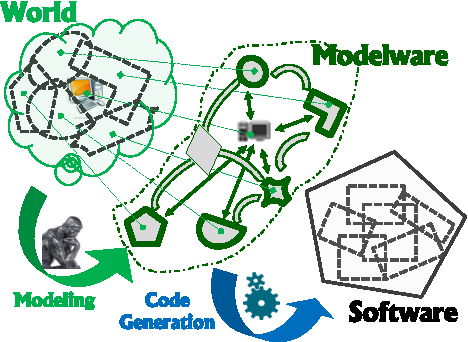
\includegraphics[width=0.5\linewidth]{mde-general}
  \caption{Общая схема MDE}
  \label{fig:mde-gen-schema}
\end{figure}

Система строится из отдельных моделей, которые представляют оригинальный объект.
Объект -- структура целостная, и его компоненты, представленные в виде моделей,
перекрывают друг друга, взаимодействуют друг с другом. Класс моделей включает
модели в виде структурных объектов отображаемых друг в друга. А это основной
феномен категорий -- функтор.

\section{Юниверсум моделей}
\label{sec:mmodcat}

Модели -- это многосортные структуры, являющиеся элементами при построении теории
\emph{метамоделей}.  Рассмотрим обобщенный вид такой теории из [39;20].
Метамодельная категория $\mathbfit{M}=(G_M,C_M)$, где $G_M$ -- граф (или более
общий вариант a priori заданного предпучка топоса $\mathbfit{G}$), а
$C_M$ -- \emph{множество ограничений} (т.е. свойства диаграммы\footnote{Специальная
  категория, в т.ч. функтор.}), заданных над $G_M$.  \emph{Экземпляром} метамодели
$\mathbfit{M}$ является пара $A = (G_A, t_A)$, где $G_A$ -- это другой граф
(объект в $\mathbfit{G}$) и $t_A: G_A \to G_M$ -- отображение (стрелка в
$\mathbfit{G}$), которую следует понимать как \emph{определение типа}, которые
удовлетворяют ограничению $A \models C_M$ (более детально в [20]).
\emph{Отображение экземпляров} $A\to B$ -- это отображение графов $f: G_A\to
G_B$, которое совместно с определением типа $f;t_B = t_A$ дает коммутативную
диаграмму.  Эти элементы задают категорию $\mathbfit{Mod}(M) \subset
\mathbfit{G}/G_M$ $M$-экземпляров.

Чтобы как-то объединить в одну структуру разрозненные гетерогенные экземпляры различных метамоделей, определим метамодельные морфизмы $m: M\to N$ как [sketch]-морфизмы,
т.е., отображения графов $m: G_M\to G_N$ совместимые по ограничениям.  Эти
отображения задают категорию $\mathbfit{MMod}$.  Теперь можно объединить все
категории $\mathbfit{Mod}(M)$ в одну категорию $\mathbfit{Mod}$, где объектами
являются экземпляры (= G-стрелки\footnote{Есть категории стрелок, но, вроде, не
  данный случай.}) $t_A: G_A\to G_{M(A)}$,
$t_B: G_B\to G_{M(B)}$ и т.д., причем каждая стрелка имеет свою метамодель, а
морфизмы $f:A\to B$ являются парами $f_{data}: G_A\to G_B$,
$f_{meta}: M(A) \to M(B)$ такие, что $f_{data};t_B = t_A; f_{meta}$, т.е.,
образуют коммутативные квадраты в $\mathbfit{G}$.  Таким образом, $\mathbfit{Mod}$
-- это подкатегория категории стрелки $\mathbfit{G}^{\to}$.

Можно показать, что [[ко]предельный] декартов квадрат (коамальгама), построенный
на действительном экземпляре $t_B: G_B\to G_N$ метамодели $N$ вдоль
[sketch]-морфизма $m:M\to N$ приводит к действительному экземпляру $M$ [20].
Таким образом определяется расслоение $\mathbfit{p} : \mathbfit{Mod} \to
\mathbfit{MMod}$, чей декартов подъем порождается этими предельными декартовыми квадратами.

\section{Трансформация моделей (MDA)}
\label{sec:mda-transform}

По большому счету MDE не интересует процесс трансформации в программный код, т.~к. интересует больше процесс внесения изменений (актуализация категории метамодели). Но в целом трансформация представляет собой последовательное уточнение описания модели до конкретных модулей, реализованных в конкретной среде программирования.

\section{Подходы к внесению изменений в модели}
\label{sec:mde-conversions}

В настоящее время выделяются два подхода к реализации трансформации --
\emph{физическое объединение моделей} и \emph{распространение изменений}.  В
первом подходе последовательно
на каждом этапе объединения из двух моделей строится одна, при этом общие
концепты сливаются в один.  Второй подход базируются на расслоении категории
метамоделей на отдельные модели, связанные друг с другом через функторы.  Эти
функторы в нотации полисистемного анализа и синтеза реализуют интерпретации
объектов и стрелок (морфизмов).

Процесс объединения моделей (первый случай) состоит из двух шагов -- а) создание
спецификации объединения, и этот этап является творческим, б) собственно
объединение, представляющее собой выполнение алгебраических операций над
моделями с целью построить общий копредел диаграммы (категорию) (см. рис.~\ref{fig:amalgama}).  Случай
аналогичный этому рассматривается в диссертации д.ф.--м.н. Ковалева Сергея
(ИДСТУ СО РАН выступал в качестве ведущей организации в 2012 году).  Основное
достоинство подхода, основанного на объединении моделей, -- это первый шаг в трансформации: в
результате объединения создается модель модуля, где все функции интегрированы в
модуль, что влечет более оптимизированный программный код (далекий от MDE пример
-- LLVM).  У С. Ковалева в качестве базовой методики проектирования выступало
аспект-ориентированное программирование, где исходными моделями для
трансформации служили амальгамы (копределы) таких объединений.  Из диссертации
не понятно было как они строились на практике, были изучены их свойства.

\begin{figure}[htbp]
  \centering
  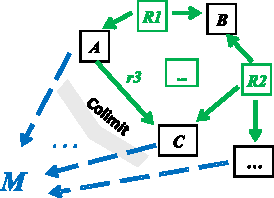
\includegraphics[width=0.5\linewidth]{amalgama}
  \caption{Построение амальгамы в процессе объединения моделей\\[0.3em]
    \footnotesize{$M$--требуемая объединенная модель, $A,B,C\ldots$ -- исходные модели.}}
  \label{fig:amalgama}
\end{figure}

Во втором случае трансформация моделей представляет собой процесс восстановление
сквозной интерпретации концептов и стрелок в расслоении, в случае, если одна из
моделей (слой) подверглась изменению.   Актуализация представляет
собой преобразование пары морфизмов (межслойная интерпретация; измененная
структура в слое, рис.~\ref{fig:propagation}) в новую пару морфизмов и распространение этой
процедуры на другие слои.  Достоинство подхода -- более естественное для
человека представление метамодельной категории (в виде слоев) и локализованная
процедура изменений (не зтрагивается все модель в целом).


\begin{figure}[htbp]
  \centering
  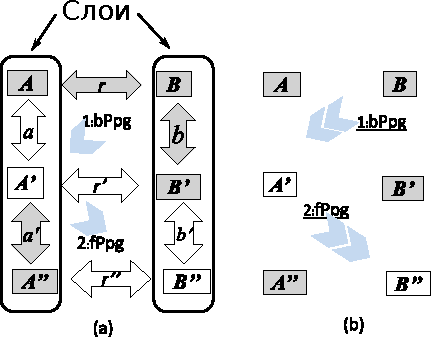
\includegraphics[width=0.5\linewidth]{propagation}
  \caption{Распространение изменений\\[0.3em]
    \footnotesize{Закрашенные фигуры -- состояние полисистемы до запуска
      процесса распространения изменений, незакрашенные -- результат процесса.
      $A',B',r'$ и т.п. -- производные объекты и отображения; $bPpg$ --
      ``обратное'' распространение изменения (морфизм $(r,b)\to (a,r')$), $fPpg$
      -- прямое ($(r',a')\to (r'',b')$).  В случае (b) перед распространением
      еще вычисляются отношения между объектами, в (a) они заданы.}}
  \label{fig:propagation}
\end{figure}


В обоих случаях присутствуют этапы, где необходимо задействовать творческий потенциал разработчика.
В первом случае -- формирование спецификации объединения, во втором -- изъятие
недостающей информации при актуализации эпиморфизмов и мономорфизмов.  Во втором
случае имеет смысл исследовать возможности компьютера в самообучении: строить
слои моделей (UML, Онтологических, Реляционных и т.п.) по мере поступления
информации от пользователя и проведения актуализации на предыдущих циклах
разработки.  Чем больше структур удастся ассимилировать, тем меньше вопросов
надо будет задавать разработчику.

\section{Построение метамодельной категории}
\label{sec:mmod-construction}

На первоначальном этапе MDE существует проблема первоначального построения
метамодельной категории, т.е. для
построения полной системы (категории) моделей необходимо выделить в предметной
области объекты и модели и построить функторы
между концептами и моделями, т.е. объекты категории метамодели $\mathbfit{MMod}$ и
морфизмы в этой категории.  В качестве методики предлагается использовать
методологию полисистемного анализа и синтеза, а метамодель строить как
полисистему.  В какой-то мере она отражена рис.~\ref{fig:propagation}b.

Разработанные процедуры распознавания концептов на примере рабочих и учебных
программ вуза -- это примеры реализации этой задачи.  По набору примеров
(абзацев), их характеристических свойств (морфизмы модели), определяется концепт
(название сущности, свойства), связь между
концептами и свойствами, а также между концептами, в нашем случае -- это
описания, последовательности и зависимости (структурные
и семантические), затем, задаются отображения этих элементов в другие слои
(например, мереологический, автоматный, логический и т.д.).  В качестве
трансформации выступает процедура представление системы модулей, всяческие
проверки на полноту (относительно требуемых в слоях отношений между
известными/распознанными концептами), генерация новых версий представлений (по
новым ФОС) и т.п.

\section{К решению задачи разработки методики построения онтологической модели предметной области}
\label{sec:technique-onto}

Здесь необходимо доделать задачу анализа процесса разработки программы,
фиксируемого в репозитариях типа GIT\@.  Задача состоит в том, чтобы в сообщениях
программистов выделить концепты и построит в слоях семантическую интерпретацию
через указание кусков кода, реализующих интерпретацию этого концепта. Для
решения этой задачи пригодится весь собранный и сконструированный инструментарий
обработки естественно-языковых текстов.

Полученные к настоящему моменту результаты (задел) опубликованы в докладе \href{http://mipro-proceedings.com/sites/mipro-proceedings.com/files/upload/cis/cis_025.pdf}{Extraction of Thesaurus and Project Structure from Linux Kernel Source Tree}.

\begin{thebibliography}{9}
\bibitem{CTMDE} Zinovy Diskin, Tom Maibaum. \emph{Category Theory and
    Model-Driven Engineering: From Formal Semantics to Design Patterns and Beyond}. Proceedings of ACCAT 2012
EPTCS 93, U. Golas, T. Soboll (Eds.), 2012, pp. 1–21, doi:10.4204/EPTCS.93.1. URL:\url{http://arxiv.org/pdf/1209.1433.pdf}.
\end{thebibliography}

% \section{Библиотека категорий, использованных в статье}
% \label{sec:catlib}

% Пусть $\mathbfit{C}$ -- категория, тогда $\mathbfit{C}^\to$ -- категория
% стрелок, состоящая из объектов $f: X\to Y$ (объектами являются морфизмы),
% морфизмов -- коммутативных квадратов
% \begin{figure}[h]
%   \centering
%   \begin{tikzpicture}
%     \node (X) {$X$};
%     \node (Y) [right of=X] {$Y$};
%     \node (Xp) [below of=X] {$X'$};
%     \node (Yp) [right of=Xp] {$Y'$};

%     \draw[->] (X) to node {$\small f$} (Y);
%     \draw[->] (Xp) to node {$\small f'$} (Yp);
%     \draw[->] (X) to node {$\small m$} (Xp);
%     \draw[->] (Y) to node {$\small n$} (Yp);
%   \end{tikzpicture}
% \end{figure}

% \noindent{}При этом $X,Y,X',Y'\in Ob(C)$, и $f,f',n,m \in Hom(C)$ ввиду того, что $n\circ
% f=f'\circ m$ (диаграмма коммутативна).

\end{document}


%%% Local Variables:
%%% TeX-master: t
%%% End:
